\documentclass{article}

\usepackage{graphicx}
\usepackage{tikz}
\usepackage{tikzsymbols}
\usetikzlibrary{calc,patterns,shapes.geometric}
\pagestyle{empty}
\usepackage[margin=0pt]{geometry}
\geometry{papersize={14in,12in}}

\def\centerarc[#1](#2)(#3:#4:#5){\draw[#1] ($(#2)+({#5*cos(#3)},{#5*sin(#3)})$) arc (#3:#4:#5);}

\begin{document}
	\begin{figure}
		\centering
		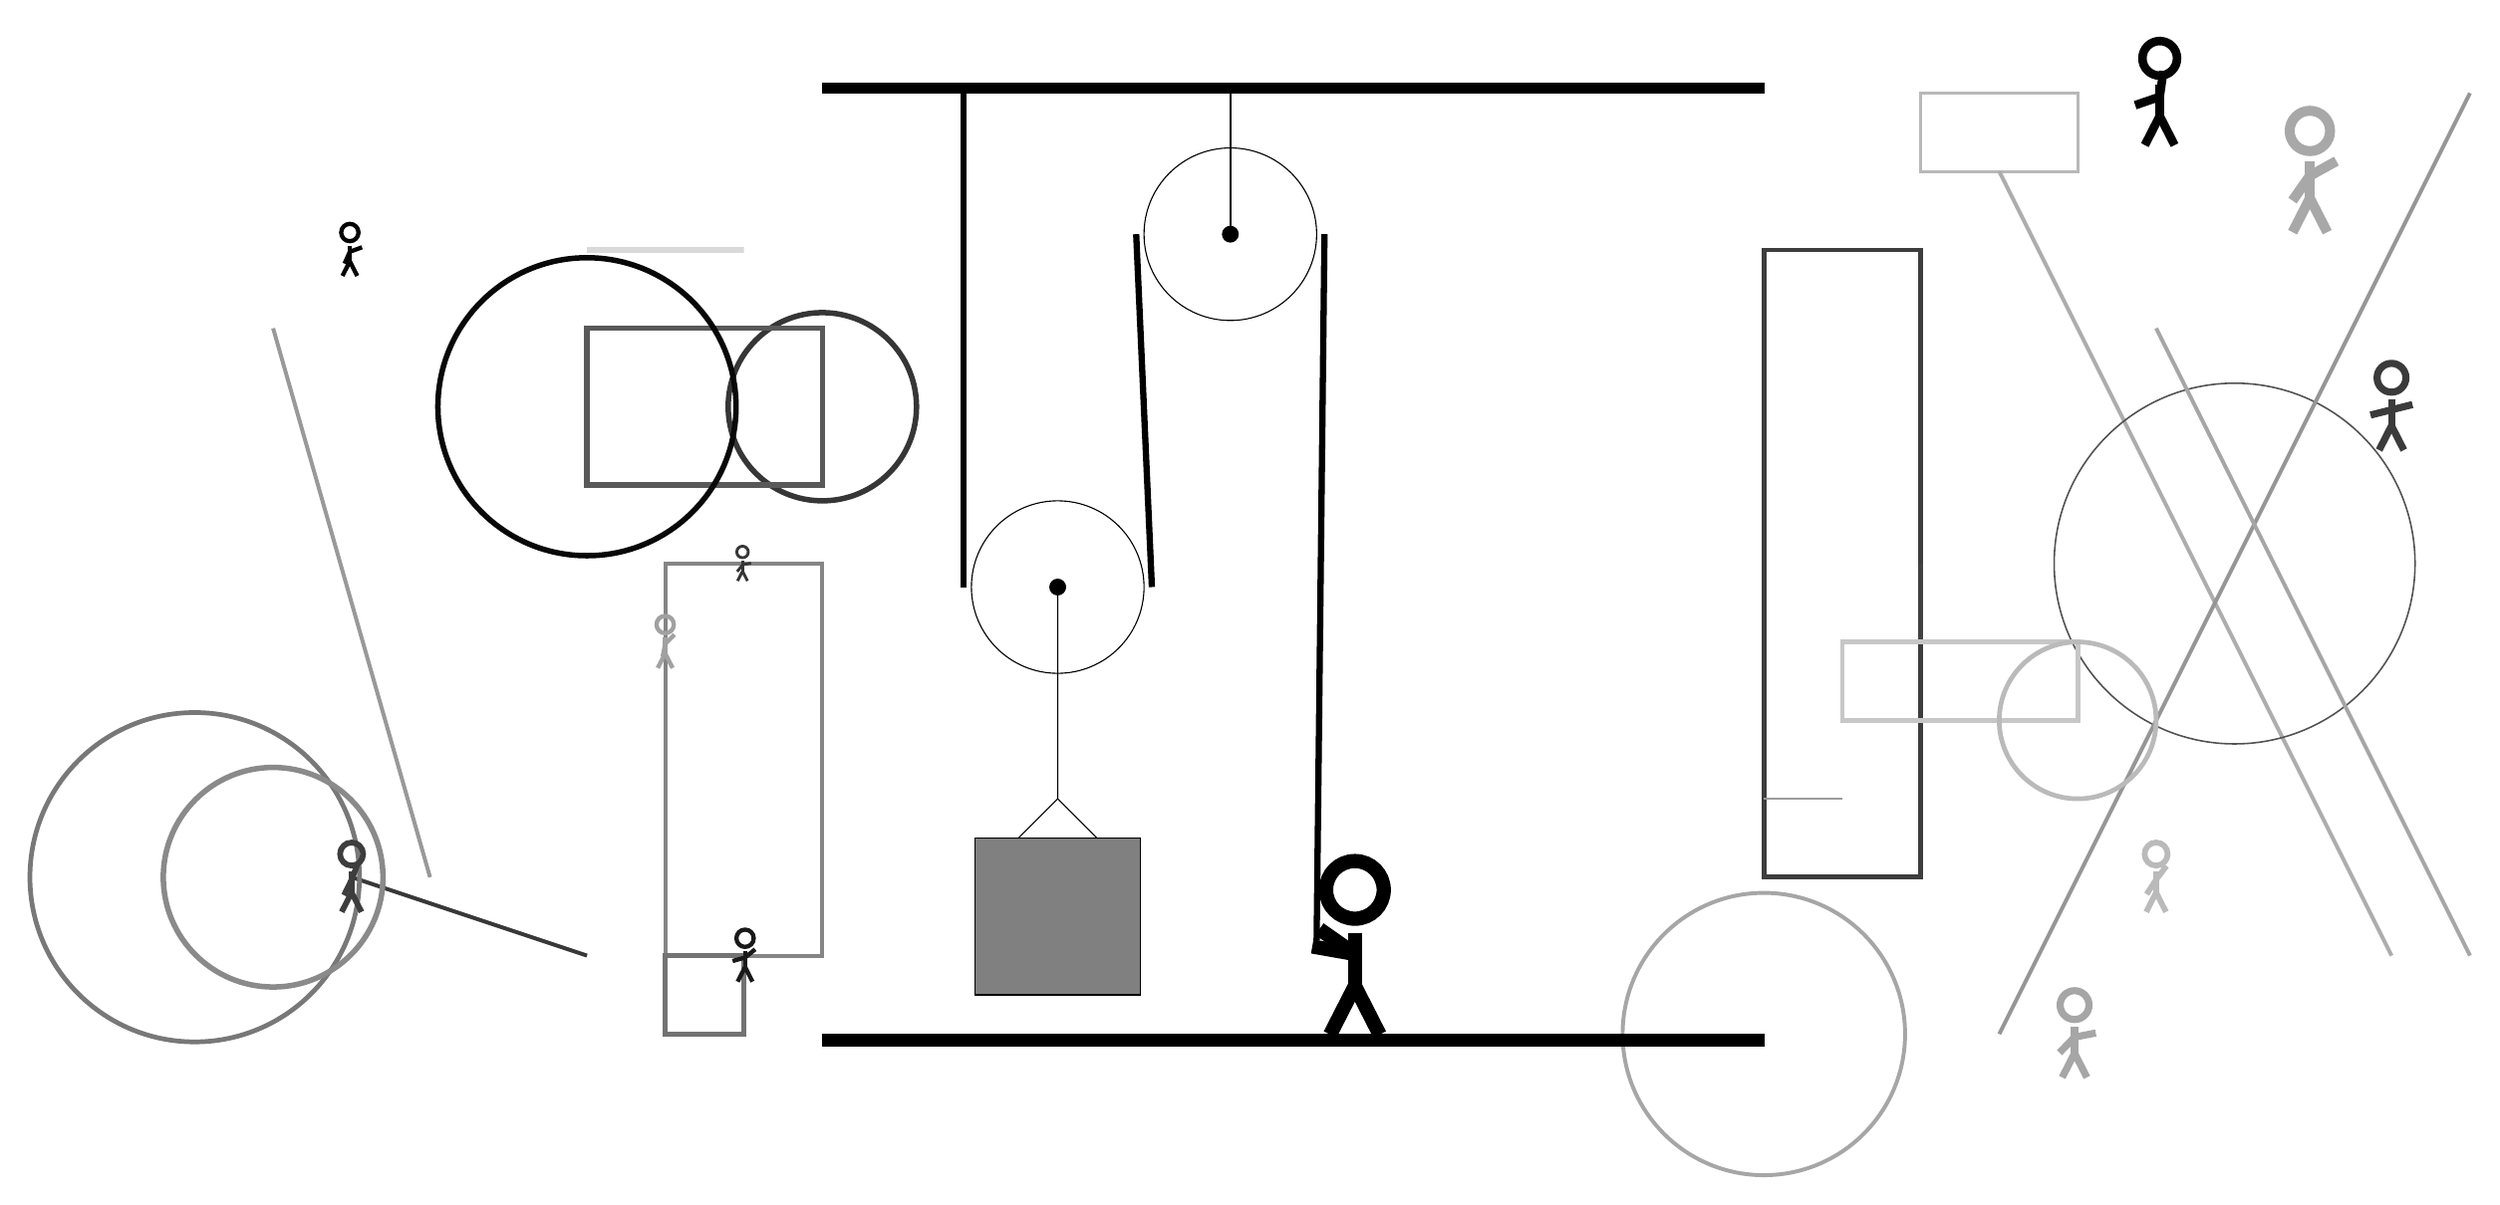
\begin{tikzpicture}
			%%%%% START %%%%%
			
			\draw[fill=black] (-2, 9) rectangle (10, 9.125);
			
			\draw (3.2, 7.2) circle (1.1);
			\draw[fill=black] (3.2, 7.2) circle (0.1);
			\draw[thick] (3.2, 7.2) -- (3.2, 9);
			
			\draw[line width=0.4mm, color=black!28] (12, 8) rectangle (14, 9);
			
			\draw [line width=0.5mm, color=black!35](10, -3) circle (1.8);
			\draw[line width=0.5mm, color=black!32](13, 8) -- (18, -2);
			\node[line width=0.6mm, color=black!99] at (-8, 7) {\Strichmaxerl[3][66][20]};
			\draw[line width=0.5mm, color=black!48] (-4, 3) rectangle (-2, -2);
			
			\draw [line width=0.7mm, color=black!79](-2, 5) circle (1.2);
			\node[line width=0.4mm, color=black!99] at (15, 9) {\Strichmaxerl[6][19][82]};
			
			\draw [line width=0.2mm, color=black!68](16, 3) circle (2.3);
			\draw[line width=0.6mm, color=black!76] (12, -1) rectangle (10, 7);
			\node[line width=0.4mm, color=black!27] at (15, -1) {\Strichmaxerl[4][57][53]};
			\draw[line width=0.3mm, color=black!39] (10, 0) rectangle (11, 0);
			\draw[line width=0.6mm, color=black!74] (12, 2) rectangle (12, 3);
			\draw[line width=0.7mm, color=black!65] (-2, 4) rectangle (-5, 6);
			
			\draw[line width=0.7mm, color=black!15] (-3, 7) rectangle (-5, 7);
			\draw[line width=0.6mm, color=black!55] (-3, -3) rectangle (-4, -2);
			\draw [line width=0.7mm, color=black!97](-5, 5) circle (1.9);
			\draw[line width=0.5mm, color=black!41](13, -3) -- (19, 9);
			
			\draw[line width=0.6mm, color=black!22] (11, 1) rectangle (14, 2);
			\draw[line width=0.5mm, color=black!78](-5, -2) -- (-8, -1);
			
			\draw [line width=0.6mm, color=black!53](-10, -1) circle (2.1);
			\node[line width=0.5mm, color=black!77] at (18, 5) {\Strichmaxerl[5][14][14]};
			\node[line width=0.2mm, color=black!35] at (14, -3) {\Strichmaxerl[5][46][11]};
			\node[line width=0.4mm, color=black!79] at (-3, 3) {\Strichmaxerl[2][52][11]};
			\node[line width=0.3mm, color=black!90] at (-3, -2) {\Strichmaxerl[3][16][39]};
			\node[line width=0.6mm, color=black!34] at (17, 8) {\Strichmaxerl[7][55][29]};
			
			\node[line width=0.5mm, color=black!37] at (-4, 2) {\Strichmaxerl[3][79][45]};
			\draw[line width=0.5mm, color=black!40](-7, -1) -- (-9, 6);
			\draw [line width=0.7mm, color=black!46](-9, -1) circle (1.4);
			
			\draw [line width=0.6mm, color=black!27](14, 1) circle (1.0);
			
			\node[line width=0.3mm, color=black!76] at (-8, -1) {\Strichmaxerl[4][64][69]};
			\draw[line width=0.5mm, color=black!35](15, 6) -- (19, -2);
			
			
			\draw (1, 2.7) circle (1.1);
			\draw[fill=black] (1, 2.7) circle (0.1);
			
			\draw (1, 2.7) -- (1, 0) -- (0.5, -0.5);
			\draw (1, 0) -- (1.5, -0.5);
			\draw[fill=black!50] (-0.05, -0.5) rectangle (2.05, -2.5);
			
			\draw[line width=0.8mm] (-0.2, 9) -- (-0.2, 2.7);
			\centerarc[line width=0.8mm](1, 2.7)(180:360:1.2000000000000002);
			\draw[line width=0.8mm](2.2, 2.7) -- (2.0, 7.2);
			\centerarc[line width=0.8mm](3.2, 7.2)(0:180:1.2000000000000002);
			\draw[line width=0.8mm](4.4, 7.2) -- (4.3, -1.8);
			
			\node at (4.7, -1.9) {\Strichmaxerl[10][-35][170]};
			
			\draw[fill=black] (-2, -3) rectangle (10, -3.15);
			
			%%%%% END %%%%%
		\end{tikzpicture}
	\end{figure}	
\end{document}